% University of Helsinki
% Department of Mathematics and Statistics
% Template for Bachelor's or Master's thesis
%
% This template is intended as a starting point for a thesis;
% feel free to customize it or use your own template.
% See the comments for hints and customization.
%
% Initial version: 29 August 2024 / Petri Laarne


% Add the 'twoside, openright' options when producing a proper printed version
\documentclass[a4paper, 11pt]{report}

\usepackage[hidelinks]{hyperref} % Always load this: clickable links and PDF reader navigation bar
\usepackage{lastpage} % Used to determine the total page count
\usepackage{calc} % For layout calculations involving TeX length units (template title page)
\usepackage{graphicx} % For embedding image files (JPEG, PNG, PDF)
\usepackage{subcaption} % For subfigures
\usepackage{tikz} % For drawing diagrams and other complex vector graphics

% If you use the LuaLaTeX or XeLaTeX compiler, comment out the following line.
% These compilers offer better support for Unicode, so you should use them if possible.
\usepackage[T1]{fontenc}
\usepackage[most]{tcolorbox}
%\DeclareAutoCiteCommand{textcite}{\textcite}{\textcites}
%\ExecuteBibliographyOptions{autocite=textcite}
\DeclareMathOperator*{\argmax}{arg\,max}

\newtcolorbox[auto counter]{proposition}[1][]{
  enhanced,
  breakable,
  fonttitle=\scshape,
  title={Proposition \thetcbcounter},
  #1
}

% Pass the language of the thesis as the LAST option in the list below.
% This changes the language used for dates and words like 'Chapter' or 'Bibliography'.
% You can remove the languages that do not appear in your work.
\usepackage[finnish,swedish,english]{babel}

\usepackage{csquotes} % This package is suggested by 'babel'

% Bibliography. Change the latter command if you modify the .bib file name.
\usepackage{biblatex}
\addbibresource{Resources/library.bib}

\usepackage{mathtools} % Extended mathematics support (this package extends amsmath)
\usepackage{amssymb} % More mathematical symbols
\usepackage{amsfonts} % Blackboard bold mathematics font

% Theorem environments
\usepackage{amsthm}
\theoremstyle{plain}
\newtheorem{theorem}{Theorem}[section] % Theorems are numbered within chapter and section
\newtheorem{lemma}[theorem]{Lemma} % Lemmas etc. follow the same numbering as theorems
\theoremstyle{definition}
\newtheorem{definition}[theorem]{Definition}
\theoremstyle{remark}
\newtheorem{remark}[theorem]{Remark}

% Some examples of custom mathematical commands
\newcommand{\ZZ}{\mathbb Z} % Blackboard bold Z
\newcommand{\RR}{\mathbb R} % Blackboard bold Z
\newcommand{\dx}{\mathop{}\!\mathrm d x} % Nice spacing (and upright d) for dx in integrals

% Finnish notation for evaluating integrals
% Instead of \int_a^b syntax you must use it as \sij{a}{b}
% (To enable the sub-/superscript syntax would require some more complicated TeX wizardry.)
\newcommand{\sij}[2]{\mathop{\bigg/}\nolimits_{\hspace{-0.65em}#1}^{\hspace{0.05em}#2}\hspace{-0.2em}}


\begin{document}

%
% TITLE PAGE
%
\begin{titlepage}

\noindent
\begin{minipage}[b]{\textwidth-45pt}
University of Helsinki\\
Faculty of Science\\
Bachelors Program in Mathematics
% Helsingin yliopisto\\
% Matemaattis-luonnontieteellinen tiedekunta\\
% Helsingfors universitet\\
% Matematisk-naturvetenskapliga fakulteten\\
\end{minipage}
\hfill
\includegraphics[width=45pt]{HYlogo.pdf}

\vspace{4pt}\hrule\vfill

\begin{center}
Bachelor's thesis\\[8pt]
% Kandidaatintutkielma / Maisterintutkielma\\[8pt]
% Kandidatavhandlingen / Magisteravhandlingen\\[8pt]

{\huge\bfseries Title of the thesis}\\[8pt]

Santeri Väätäjä
\end{center}

\vfill\hrule\vspace{4pt}

\noindent
Supervisor:\hfill Month and year of submission\\
Petri Ola\\
\end{titlepage}

%
% ABSTRACT
%
% This command starts a new page.
% In a print version ('twoside' option passed to \documentclass), the page is on the right side
\pagenumbering{gobble}
\cleardoublepage

\noindent\textbf{Title:} Repeat the title here\\ % Otsikko / Titel
\textbf{Author:} Santeri Väätäjä\\ % Tekijä / Författare
\textbf{Month and year:} Month and year of submission\\ % Aika / Datum
\textbf{Page count:} \pageref*{LastPage}~pp.\\[1em] % Sivumäärä: XX~s. / Sidoantal: XX~s.
% The page count is updated automatically, but it might require two compilations to be correct.
% If you customize the backmatter, this might become incorrect - check and correct manually if needed.

% If you include an abstract in a different language, wrap it in a foreignlanguage block
\begin{foreignlanguage}{english}
\noindent\textbf{Abstract:}\\ % Tiivistelmä / Referat
The abstract should be about one page long.
It also doubles as the maturity test.
Do not use mathematical notation in the abstract,
since it will also be displayed on the electronic thesis repository.

For the publication date, put in the month and year of submission of the finished thesis.
Also include 3~to 5~keywords that support searching for your thesis.
They are also shown one the repository page.

You can include the abstract in more than one language by copying and modifying
this code between comment blocks.
To get correct hyphenation for the language (and not with the rules of the main language),
put the text in a \verb|foreignlanguage| block as shown in the code
(just modify the language parameter to match the abstract).
\end{foreignlanguage}


\vfill

\noindent\textbf{Keywords:} Fill in some keywords, Separated by commas % Avainsanat / Nyckelord




%
% TABLE OF CONTENTS
%
\cleardoublepage
\tableofcontents


%
% MAIN TEXT STARTS HERE
%

% The \pagenumbering{arabic} command must be immediately after the first chapter title.
% Do not repeat it for other chapters.
\chapter{Introduction}
\pagenumbering{arabic}

\chapter{Poisson Kernel in $\RR_+^{n+1}$}
In order to define the Poisson kernel

%\begin{definition}[Summability to $L$]\label{def:mean_of_int}
%    A function $f$ is said to be $M$-summable to $L$, if $\lim_{\epsilon\rightarrow0}M_{\epsilon,\Phi}(x)=L$, where
%
%    \begin{equation*}
%        M_{\epsilon,\Phi}(f)=M_{\epsilon}(f)=\int_{\RR^n}\Phi(\epsilon x)f(x)dx
%    \end{equation*}

%    \noindent where $\Phi\in C_0$ and $\Phi(0)=1$. Then $M_\epsilon(f)$ is called the $\Phi$-mean of the integral.
%\end{definition}

\clearpage
\chapter{Harmonic functions in $E_+^{n+1}$}

This chapter will consider the main result of the Dirichlet problem in the half-space for Laplace's equation. I will only consider here the tangential convergence, where the limit is taken tangentially towards the boundary value. All of this chapter follows closely the results by Stein and Weiss from \cite{stein_weiss}.

I will start the chapter by first introducing some new, necessary constructs that are used in the main result: Theorem \ref{thm:2.3}. This result, together with Theorem \ref{thm:21a}, provides a way to lift the problem from the boundary $\RR^n$ to the half space $\RR^{n+1}_+$, where the extension is harmonic; consequently, the results from harmonic functional analysis apply to the problem. First, Theorem \ref{thm:21a} will show that $L^p$ functions behave as desired, and the Poisson integral converges towards the function at the boundary $\RR^n\times\{0\}$. Then Theorem \ref{thm:2.3} will extend this result to apply to a broader class of finite Borel measures.

These results need some additional concepts to be understood. Therefore, in the second Section definition of the total variational measure and the norm induced by that are defined. Also, to prove Theorem \ref{thm:2.3}, a weaker notion of convergence is needed, and for this purpose, the weak$^*$ convergence is introduced.

\section{The Characterization of Poisson Integral for $L^p$-space}\label{sec:LP}

In this section, I will concentrate on the version of Dirichlet's problem where the data\textemdash meaning the function towards which the harmonic function converges at the boundary of a half space\textemdash belongs to the $L^p$ space. Main results of this section, Theorems \ref{thm:21a} and \ref{thm:21b} will be concerned with recovering the boundary value function by extending it to the half space through the Poisson integral. These also establish a regularity for the Poisson integral and show that it also belongs to the $L^p$ space.

Proofs for these theorems require some preliminary results. These are introduced before the main results. These results show that the convolutions of $L^p$ functions with functions that resemble good kernels as approximate identities will converge, in some cases pointwise and in other cases in the $L^p$ sense, to the function against which it is convoluted.

The first of these results shows convergence in the $L^p$ sense.

\begin{lemma}\label{lemma:118}
    Suppose $\phi\in L^1(\RR^n)$ with $\int_{\RR^n}\phi(x)dx=1$ and for $\epsilon>0$ let $\phi_\epsilon(x)=\epsilon^{-n}\phi(x/\epsilon)$. If $f\in L^p(\RR^n)$ for some $1\leq p<\infty$, or $f\in C_0\subset L^\infty(\RR^n)$, then $\|f*\phi_\epsilon-f\|_p\rightarrow0$ as $\epsilon\rightarrow0$. In particular, $u(x,\epsilon)=\int_{\RR^n}f(t)P(x-t,\epsilon)dt$ and $s(x,\epsilon)=\int_{\RR^n}f(t)W(x-t,\epsilon)dt$ converge to $f$ in the $L^p$ norm as $\epsilon\rightarrow0$.
\end{lemma}
\begin{proof}
    By change of variables
    \begin{equation*}
        \int_{\RR^n} \phi_{\epsilon}(t)dt=\int_{\RR^n} \epsilon^{-n}\phi(t/\epsilon)dt=\int_{\RR^n} \phi(t)dt=1
    \end{equation*}
    and therefore
    \begin{equation*}
        (f*\phi_\epsilon)(x)-f(x)=\int_{\RR^n}(f(x-t)-f(x))\phi_\epsilon(t)dt.
    \end{equation*}
    Then by Minkowski's integral inequality
    \begin{align*}
        \|f*\phi_\epsilon-f\|_p&\leq\int_{\RR^n}\left(\int_{\RR^n}|f(x-t)-f(x)|^pdx\right)^{\frac{1}{p}}\epsilon^{-n}|\phi(t/\epsilon)|dt \\
        &=\int_{\RR^n}\left(\int_{\RR^n}|f(x-\epsilon t)-f(x)|^pdx\right)^{\frac{1}{p}}|\phi(t)|dt
    \end{align*}
    where $\omega(h)=\left(\int_{\RR^n}|f(x-h)-f(x)|^pdx\right)^{\frac{1}{p}}$ is the $L^p$ modulus of continuity of $f$. Since $\omega(h)\leq2\|f\|_p$ the modulus is bounded. Additionally, as $h\rightarrow0$ also $\omega(h)\rightarrow0$ when $f\in C_0$. If $f\in L^p(\RR^p)$, since $C_0$ is dense in $L^p$, the function can be approximated by some $f_c$ that belongs to $C_0$, and therefore
    \begin{equation*}
        \|f*\phi_\epsilon-f\|_p\leq\int_{\RR^n}\omega(-\epsilon t)|\phi(t)|dt.
    \end{equation*}
    By dominated convergence, the right-hand side of the equation tends to zero as $\epsilon\rightarrow0$, as $\omega(-\epsilon t)|\phi(t)|\leq2\|f\|_p|\phi(t)|$, proving the lemma.
\end{proof}

For the purposes of the second result, the concept of Lebesgue point and Lebesgue set is needed. These provide a generalization of continuity to $L^p$ spaces where we do not have pointwise control of a function, and therefore, continuity as such cannot be enforced. 

\begin{definition}
    Let $f$ be locally integrable. Then the set that is formed by $x$'s such that
    \begin{equation*}
        \frac{1}{r^n}\int_{|t|<r}|f(x-t)-f(x)|dt\rightarrow0
    \end{equation*}
    as $r\rightarrow0$, is called the Lebesgue set of $f$.
\end{definition}

Lebesgue sets are now used in the next result to show that pointwise convergence of the Poisson integral can also be established under certain conditions for almost every $x\in\RR^n$. 

\begin{lemma}\label{lemma:125}
    Suppose $\phi\in L^1(\RR^n)$. Let $\psi(x)=\mathrm{ess. sup}_{|t|\geq|x|}|\phi(t)|$ and, for $\epsilon>0$, let $\phi_\epsilon(x)=\epsilon^{-n}\phi(x/\epsilon)$. If $\psi\in L^1(\RR^n)$ and $f\in L^p(\RR^n)$ for some $1\leq p\leq\infty$, then $\lim_{\epsilon\rightarrow0}(f*\phi_\epsilon)(x)=f(x)\int_{\RR^n}\phi(t)dt$ whenever $x$ belongs to the Lebesgue set of $f$. In particular, the Poisson and Gauss-Weierstrass integrals of $f$, $\int_{\RR^n}f(t)P(x-t,\epsilon)dt$ and $\int_{\RR^n}f(t)W(x-t,\epsilon)dt$, converge to $f(x)$ as $\epsilon\rightarrow0$ for almost every $x\in\RR^n$.
\end{lemma}
\begin{proof}
    Let $x$ be a fixed point in the Lebesgue set of $f$ and $\delta>0$. Then for some $\eta>0$ holds
    \begin{equation}\label{eq:cond-i}
        r^{-n}\int_{|t|<r}|f(x-t)-f(x)|dt<\delta
    \end{equation}
    whenever $r\leq\eta$.
    
    Let $a=\int_{\RR^n}\phi_\epsilon(t)dt$. Then for all $\epsilon>0$
    \begin{align*}
        |(f*\phi_\epsilon)(x)-af(x)|&=\left|\int_{\RR^n}(f(x-t)-f(x))\phi_\epsilon(t)dt \right| \\
        &\leq \left|\int_{|t|<\eta}(f(x-t)-f(x))\phi_\epsilon(t)dt \right|+\\
        &\quad\,\left|\int_{|t|\geq\eta}(f(x-t)-f(x))\phi_\epsilon(t)dt \right| \\
        &=I_1 + I_2
    \end{align*}
    This splits the analysis into two cases. The first one considers points that are close to the $x$ and the second gives a tail estimate for values that are further. 
    
    To estimate $I_1$ it is possible to use the assumption that $x$ belongs to the Lebesgue set. Let $\psi_0(r)=\psi(|x|)$ be the radial function generated from $\psi$. It is a decreasing function of $r$. Thus for $\Omega_n$, denoting the volume of solid unit sphere of $\RR^n$
    \begin{equation*}
        \frac{\Omega_n(2^n-1)}{2^n}r^n\psi_0(r)\leq\int_{r/2\leq|x|\leq r} \psi(x)dx\rightarrow0
    \end{equation*}
    as $r\rightarrow 0$, or $r\rightarrow\infty$. Thus there exists a constant $A$ such that for $0<r<\infty$ $r^n\psi_0(r)\leq A$. Let $\Sigma_{n-1}$ denote the surface of the unit sphere in $\RR^n$ and $g(r)=\int_{\Sigma_{n-1}}|f(x-r\sigma)-f(x)|d\sigma$, where $\sigma$ is the surface are element of $\Sigma_{n-1}$. Then, by a change of variable, Equation \ref{eq:cond-i} is equivalent to
    \begin{equation*}
        G(r)=\int_0^rs^{n-1}g(s)ds\leq\delta r^n
    \end{equation*}
    when $r\leq\eta$. By using $G(r)$ we can further analyze the integral $I_1$.
    \begin{align}\label{eq:I1}
        \begin{split}
            I_1&=\left|\int_{|t|<\eta}(f(x-t)-f(x))\phi_\epsilon(t)dt \right| \\
            &\leq\int_{|t|<\eta}|f(x-t)-f(x)|\epsilon^{-n}\phi(t/\epsilon)dt \\
            &=\int_0^\eta r^{n-1}g(r)\epsilon^{-n}\psi_0(r/\epsilon)dr \\
            &=[G(r)\epsilon^{-n}\psi_0(r/\epsilon)]_0^\eta-\int_0^\eta G(r)\epsilon^{-n}d\psi_0(r/\epsilon) \\
            &\leq[\delta r^n\epsilon^{-n}\psi_0(r/\epsilon)]_0^\eta-\int_0^{\frac{\eta}{\epsilon}}G(\epsilon s)\epsilon^{-n}d\psi_0(s) \\
            &\leq\delta A-\int_0^{\frac{\eta}{\epsilon}}\delta s^nd\psi_0(s) \\
            &\leq\delta\left(A-\int_0^\infty s^nd\psi_0(s) \right)
        \end{split}
    \end{align}
    Then by doing the change of variables from radial $\psi_0$ back to the Euclidean space, as $dx=r^{n-1}drd\sigma$ the last row of equation \ref{eq:I1} can be integrated by using integration by parts and the fact that $\psi_0(s)\rightarrow0$ as $s\rightarrow0$ or $s\rightarrow\infty$.
    \begin{align*}
        -\int_0^\infty s^nd\psi_0(s)&=n\int_0^\infty s^{n-1}\psi_0(s) ds-[s^n\psi_0(s)]_0^\infty \\
        &=n\int_0^\infty s^{n-1}\psi_0(s) ds \\
        &=\frac{n}{\omega_{n-1}}\int_{\RR^n}\psi(x)dx
    \end{align*}
    This shows that $I_1$ is bounded by a constant $\delta B$.

    The tail estimate $I_2$ can be analyzed by using Hölder's inequality for $1/p+1/p'=1$.
    \begin{align}\label{eq:I2}
        \begin{split}
            I_2&=\left|\int_{|t|\geq\eta}(f(x-t)-f(x))\phi_\epsilon(t)dt \right| \\
            &\leq\int_{|t|\geq\eta}|f(x-t)-f(x)|\phi_\epsilon(t)dt \\
            &\leq\int_{|t|\geq\eta}(|f(x-t)|\phi_\epsilon(t)+|f(x)|\phi_\epsilon(t))dt \\
            &\leq\|f\|_p\|\phi_\epsilon\chi_{\{|t|\geq\eta\}}\|_{p'}+|f(x)|\|\phi_\epsilon\chi_{\{|t|\geq\eta\}}\|_{1}
        \end{split}
    \end{align}
    Where
    \begin{equation*}
        \|\phi_\epsilon\chi_{\{|t|\geq\eta\}}\|_{1}=\int_{|t|\geq\eta}\phi_\epsilon(t)dt=\int_{|t|\geq\eta/\epsilon}\phi(t)dt
    \end{equation*}
    so the second term in the equation \ref{eq:I2} tends to zero at the same time as $\epsilon$. 
    
    The same is also true for the second term. For $p$ and $p'$ holds the following relationship: $p'=1+p'/p$. Then, by Hölder's inequality applied to the first term gives
    \begin{align*}
        \|\phi_\epsilon\chi_{\{|t|\geq\eta\}}\|_{p'}&=\left(\int_{|t|\geq\eta}\phi_\epsilon(t)^{p'}dt \right)^{\frac{1}{p'}} \\
        &=\left(\int_{|t|\geq\eta}\phi_\epsilon(t)^{\frac{p'}{p}}\phi_\epsilon(t) dt \right)^{\frac{1}{p'}} \\
        &\leq\|\phi_\epsilon\chi_{\{|t|\geq\eta\}}\|_{\infty}^{\frac{1}{p}}\|\phi_\epsilon\chi_{\{|t|\geq\eta\}}\|_{1}^{\frac{1}{p'}}
    \end{align*}
    However, $\|\phi_\epsilon\chi_{\{|t|\geq\eta\}}\|_\infty=\epsilon^{n}\psi(\eta/\epsilon)$, which goes to zero as $\epsilon$ goes zero. 
    
    Therefore, as $\epsilon$ tends to zero, $I_2$ also tends to zero and $I_1$ is bounded by some constant $\delta B$ where the $\delta$ depends on $\psi$. Consequentially also the difference $|(f*\phi_\epsilon)(x)-f(x)|\rightarrow0$.
\end{proof}

Now we have all of the results that are needed for the convergence of the Poisson integral. The last preliminary result for the main theorems of this section provides one more inequality that is used to bound the norm of the Poisson integral with respect to the boundary value function.

\begin{lemma}\label{lemma:conv-lp}
    If $f\in L^p(\RR^n)$, $1\leq p\leq\infty$, and $g\in L^1(\RR^n)$ then $h=f*g=\int_{\RR^n}f(x-t)g(t)dt$ is well defined and belongs to $L^p(\RR^n)$. Also,
    \begin{equation*}
        \|h\|_p\leq\|f\|_p\|g\|_1.
    \end{equation*}
\end{lemma}
\begin{proof}
    By Minkowski's integral inequality, we have
    \begin{align*}
        \|h\|_p&=\left(\int_{\RR^n}\left|\int_{\RR^n}f(x-t)g(t)dt\right|^pdx\right)^{\frac{1}{p}} \\
        &\leq\int_{\RR^n}\left(\int_{\RR^n}|f(x-t)|^pdx\right)^{\frac{1}{p}}|g(t)|dt \\
        &=\int_{\RR^n}\|f(\cdot-t)\|_pg(t)dt \\
        &\leq\|f\|_p\|g\|_1
    \end{align*}
    so also $h\in L^p(\RR^n)$.
\end{proof}

Finally, all the required results are established, and it is possible to prove the main theorems in this section. These results will show that the Poisson integral acts as a natural harmonic extension for a function in $L^p$ into the half space. It gives the conditions under which a function $f$ that is defined over $\RR^n$ can be recovered from the boundary of a harmonic function defined over one dimension higher half space $\RR^{n+1}_+$.

\begin{theorem}\label{thm:21a}
    If $f\in L^p(\RR^n)$, $1\leq p\leq\infty$ and
    \begin{equation*}
        u(x,y)=\int_{\RR^n}f(t)P(x-t,y)dt
    \end{equation*}
    is the Poisson integral of $f$ then $u$ is harmonic in $\RR_+^{n+1}$, converges towards the function $f$ at the boundary of half space $\lim_{y\rightarrow0}u(x,y)=f(x)$ for almost every $x\in\RR^n$ and
    \begin{equation}\label{eq:lemma21a-ineq}
        \|u(\cdot,y)\|_p\leq\|f\|_p
    \end{equation}
    for all $y>0$. If $1\leq p<\infty$ then
    \begin{equation*}
        \|u(\cdot,y)-f\|_p\rightarrow0
    \end{equation*}
    as $y\rightarrow0$. That is, $u(\cdot,y)$ converges to $f$ in the $L^p$ norm as $y\rightarrow0$.
\end{theorem}
\begin{proof}
    The Poisson integral can be shown to be harmonic by showing that $\Delta_{x,y} u(x,y)=0$. Since the Poisson kernel is harmonic, this could be shown by taking the Laplace operator inside the integral. Let $y>0$, then from the equation \ref{eq:d2dx2P} the absolute value of the second derivative with respect to $x_i$ can be bounded as:
    \begin{align*}
        \left|\frac{\partial^2P(x,y)}{\partial x_i^2}\right| &=\left|c_n(n+1)y\left( \frac{(n+3)x_i^2}{(y^2+|x|^2)^\frac{n+5}{2}}-\frac{1}{(y^2+|x|^2)^\frac{n+3}{2}}\right)\right| \\
        &= \left|c_n(n+1)y\left( \frac{(n+3)x_i^2}{(y^2+|x|^2)^\frac{n+5}{2}}-\frac{y^2+|x|^2}{(y^2+|x|^2)^\frac{n+5}{2}}\right)\right| \\
        &\leq c_n(n+1)y\frac{(n+2)(y^2+|x|^2)}{(y^2+|x|^2)^\frac{n+5}{2}} \\
        &=\frac{C_n^x}{(y^2+|x|^2)^\frac{n+3}{2}}.
    \end{align*}
    The second derivative of $P$ with respect to $y$ from the equation \ref{eq:d2dyP} can be bounded similarly.
    \begin{equation*}
        \left|\frac{\partial^2P(x,y)}{\partial y^2}\right|\leq \frac{C_n^y}{(y^2+|x|^2)^\frac{n+3}{2}}
    \end{equation*}
    Therefore, the dominated convergence applies to the Poisson integral and allows for the change of order in integration and differentiation. By using this and the Poisson kernels' harmonicity, the integral is shown to be harmonic.
    \begin{align*}
        \Delta_{x,y} u(x,y)&=\Delta_{x,y}\int_{\RR^n} P(x-t,y)f(t)dt \\
        &=\int_{\RR^n} \Delta_{x,y}P(x-t,y)f(t)dt \\
        &=\int_{\RR^n} 0\cdot f(t)dt \\
        &=0
    \end{align*}
    
    The limit of the Poisson integral $\lim_{y_\rightarrow0}u(x,y)=f(x)$ for almost every $x$, follows from the Lemma \ref{lemma:125}.

    Similarly, $L^p$ convergence $\|u(\cdot,y)-f\|_p$ follows from the Lemma \ref{lemma:118}.

    Finally, the inequality \ref{eq:lemma21a-ineq} is a direct consequence of Lemma \ref{lemma:conv-lp}, where $g(x)=P(x,y)$ and the convolution corresponds to the Poisson integral $u(x,y)$.

    These prove the lemma.
\end{proof}

Figure \ref{fig:convergence} shows Theorem \ref{thm:21a} in action. In the example, the domain is not exactly the half space, but a subspace of it, as the integration is done only in the $[0,2\pi]$ interval and therefore the Poisson integral is only showing a subset of $[0,2\pi]\times\RR_+$.

\begin{figure}[h]
\centering
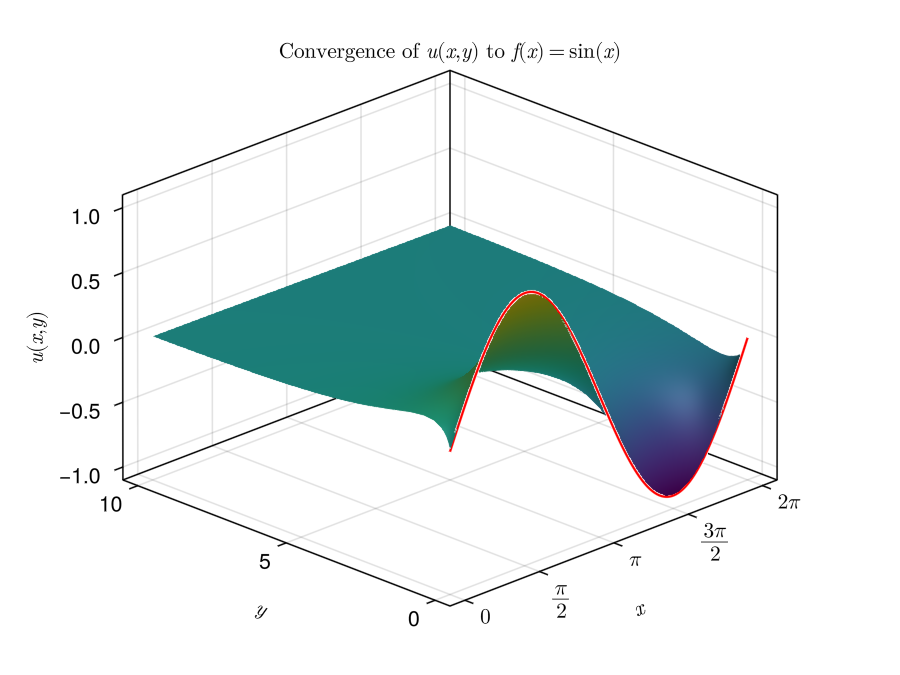
\includegraphics[width=\textwidth]{Figures/convergence.png}
\caption{Convergence of Poisson integral $u(x,y)=\int_0^{2\pi}P(x-t,y)\sin(t)dt$ to $f(x)=\sin(x)$, which is shown as the red line, in 2-dimensional subspace $[0,2\pi]\times\RR_+$.}
\label{fig:convergence}
\end{figure}

The next result will strengthen the result of Theorem \ref{thm:21a} when stricter regularity assumptions are applicable for the boundary value function $f$. It shows that in specific cases where it is assumed to be continuous and bounded, the convergence of the Poisson integral accepts a stronger convergence result, as it is shown to converge uniformly in this case.

\begin{theorem}\label{thm:21b}
    If $f\in C_0\subset L^p(\RR^n)$ then the Poisson integral of $f$, $u(x,y)$, converges to f uniformly: $\|u(\cdot,y)-f\|_\infty=\sup_{x\in\RR^n}|u(x,y)-f(x)|\rightarrow0$ as $y\rightarrow0$. 
    
    If the function $f$ is only assumed to be continuous and bounded, the convergence is uniform on compact subsets of $\RR^n$. In either case, we can exted $u(x,y)$ to $\Bar{\RR^{n+1}_+}=\RR_+^{n+1}\cup\RR^n$ by letting $u(x,0)=f(x)$ and we obtain a continuous function.
\end{theorem}
\begin{proof}
    If $f\in C_0\subset L^\infty$, the Poisson integral $u(x,y)$ converges to $f(x)$ as $y\rightarrow0$, as every point belongs to the Lebesgue set of $f$ and Lemma \ref{lemma:125} holds.

    To establish uniform convergence in a compact subset $K\subset\RR^n$, let $\epsilon>0$, then there exists $\delta>0$ such that $|f(x-t)-f(x)|<\epsilon$ if $x\in K$ and $|t|<\delta$. Therefore
    \begin{align*}
        |u(x,y)-f(x)|&=\left|\int_{\RR^n}f(x-t)P(t,y)dt- f(x) \right| \\
        &\leq\int_{|t|\leq\delta}\left|f(x-t)-f(x)\right|P(x,t)dt+ \\
        &\quad\,\int_{|t|>\delta}\left|f(x-t)-f(x)\right|P(x,t)dt \\
        &\leq\epsilon\int_{\RR^n}P(t,y)+2\|f\|_\infty\int_{|t|>\delta}P(t,y)dt \\
        &=\epsilon+2\|f\|_\infty\int_{|t|>\delta}P(t,y)dt
    \end{align*}
    For fixed $\delta$, $\int_{|t|>\delta}P(x,y)dt\leq c_ny\int_{|t|>\delta}|t|^{-n-1}dt\rightarrow0$ as $y\rightarrow0$. Thus $|u(x,y)-f(x)|\leq\epsilon$ when $y$ gets close to zero, for all $x\in K$. If $f\in C_0$, then $f$ is also uniformly continuous and for $\delta$ exists $|f(x-t)-f(x)|<\epsilon$ for all $x\in\RR^n$ as $|t|<\delta$. Therefore, $u$ converges uniformly towards $f$ as $y\rightarrow0$, and the claim of the lemma is proved.
\end{proof}

This section showed that the Poisson integral characterizes the harmonic function in the half space $\RR^{n+1}_+$ that converges towards the boundary value function. Theorem \ref{thm:21b} additionally showed that by assuming more regularity for the boundary data, it is also possible to get stronger convergence results.

These results could be used, for example, as a tool to solve certain problems in PDEs. Most straightforward applications consider, of course, the Laplace equation in the Euclidean half space as if one is trying to solve a problem of the form:
\begin{equation*}
    \Delta u=0\text{ in }\RR^{n+1}_+\text{, and }\lim_{y\rightarrow0}u(x,y)=f(x).
\end{equation*}
These results show that the Poisson integral will give the solution that is sought.

However, the result is applicable to a wider range of problems than this. The natural next step from here could be to consider the heat equation $u_t=\Delta u$, which has the Laplace's equation as a steady state equilibrium. To solve it for an initial data $u(x,0)=f(x)$, the techniques that were developed in the theorems of this section could also be used.

\section{The Characterization of Poisson-Stiltjes Integral for the Space of Finite Borel Measures $\mathcal M$}

After considering $L^p$ functions in Section \ref{sec:LP} and proving the Poisson integral converges to a $L^p$ function at the boundary of a half space, it is possible to widen the scope and consider a similar problem in other spaces. In this section, $L^p$ functions are replaced by measures, especially finite Borel measures. The convergence result with finite Borel measures is otherwise very similar to Theorem \ref{thm:21a}, but some definitions change due to the move from $L^p$ functions to finite Borel measures $\mathcal M$.

First of all, the measure $\mu\in\mathcal M(\RR^{n})$ requires a new definition for the norm. For this purpose, we need the total variation. The total variation of a measure is a positive measure defined by another measure as follows. 

\begin{definition}[Total Variation Measure]
    Let $\mu$ be a measure on measurable space $(X,\mathcal{S})$. The total variation measure is the function $|\mu|:\mathcal{S}\rightarrow [0,\infty]$ that is defined by
    \begin{align*}
        |\mu|(E) =\sup\{&|\mu|(E_1)+\ldots+|\mu|(E_m)|\\
        &m\in\mathbb{N}, E_1,\ldots,E_m\text{ are disjoint and }E_1,\ldots,E_m\subset E\}.
    \end{align*}
    for $E\subset X$. The total variation norm $\|\mu\|=|\mu|(X)$ is the total variation measure throughout the space.
\end{definition}

The total variation is a measure, and the total variation norm is a norm as provided in \cite{axler_measure_2019}. The total variation of a measure can be seen as an extension of the concept of absolute value to measures from functions. It attempts to encode the ``size'' of a measure by disregarding the sign.

As the convergence concept used in theorem \ref{thm:21a} was $L^p$ convergence in the norm, that is also out of question now. For that reason, a new type of convergence is introduced.

\begin{definition}[Weak* convergence]
    Let $X$ be a normed linear space, and suppose that $\mu_n,\mu\in X^*$, where $X^*$ is the dual space of the normed space $X$. Then $\mu_n$ is said to converge weak* if
    \begin{equation*}
        \forall x\in X,\quad\lim_{n\rightarrow\infty}\langle x,\mu_n\rangle=\langle x,\mu\rangle.
    \end{equation*}
\end{definition}

These are enough to acquire a similar result for finite Borel measures as for $L^p$ functions. The next theorem shows this result. 

\begin{theorem}\label{thm:2.3}
    If $\mu\in\mathcal M(\RR^{n})$ and $u(x,y)=\int_{\RR^n}P(x-t,y)d\mu(t)$ is the Poisson-Stiltjes integral of $\mu$ then $u$ is harmonic in $\RR_+^{n+1}$ and 

    \begin{equation}\label{eq:main-ineq}
        ||u(\cdot,y)||_1=\int_{E_n}|u(x,y)|dx\leq||\mu||
    \end{equation}

    \noindent where $||\mu||$ is the total variation, $|\mu|(\RR_n)$, of $\mu$. Furthermore,

    \begin{equation}\label{eq:main-convergence}
        \lim_{y\rightarrow0}\int_{E_n}u(x,y)\varphi(x)dx=\int_{E_n}\varphi(x)d\mu(x)
    \end{equation}

    \noindent for all $\varphi\in C_0$; that is, $u(\cdot,y)$ converges to $\mu$ in the weak* topology.
\end{theorem}
\begin{proof}
    The Poisson-Stiltjes integral can be shown to be harmonic in an analogous way to the Poisson integral. The analysis concerning Poisson kernels' second derivatives does not change, and therefore, the dominated convergence can also be used in this instance. Then the result is acquired by the same change of order in integration and differentiation.
    \begin{align*}
        \Delta_{x,y} u(x,y)&=\Delta_{x,y}\int_{\RR^n}P(x-t,y)d\mu(t) \\
        &=\int_{\RR^n}\Delta_{x,y}P(x-t,y)d\mu(t) \\
        &=\int_{\RR^n}0\cdot d\mu(t) \\
        &=0
    \end{align*}

    The inequality \ref{eq:main-ineq} now follows from the Lemma \ref{lemma:conv-lp} by changing the $L^1$ function $g$ to a Borel measure $\mu\in\mathcal M(\RR^n)$ and applying the total variation to the expression $h(x)=\int_{\RR^n}f(x-t)d\mu(t)$. Minkowski's integral inequality can be applied to the norm to obtain that $\int_{\RR^n}|u(x,y)|dx\leq\int_{\RR^n}\|u(\cdot,y)\|_1d\mu(t)$. Since $\int_{\RR^n}P(x,y)dx=1$, this leads to the inequality \ref{eq:main-ineq}.

    The weak* convergence still remains to be proven. In order to prove that, suppose $v(x,y)=\int_{\RR^n}P(x-t,y)\varphi(x)dx$ i.e., $v(x,y)$ is $\varphi(x)$s Poisson integral. Then the equation \ref{eq:main-convergence} can be written as
    \begin{align*}
        \int_{\RR^n}u(x,y)\varphi(x)dx&=\int_{\RR^n}\left(\int_{\RR^n}P(x-t,y)d\mu(t)\right)\varphi(x)dx \\
        &=\int_{\RR^n}\left(\int_{\RR^n}P(x-t,y)\varphi(x)dx\right)d\mu(t) \\
        &=\int_{\RR^n}v(t,y)d\mu(t)
    \end{align*}
    which allows the use of Theorem \ref{thm:21b} for the $C_0$ function $\varphi$ and its Poisson integral $v$.
    \begin{align*}
        \left|\int_{\RR^n}u(x,y)\varphi(x)dx-\int_{\RR^n}\varphi(t)d\mu(t)\right|&=\left|\int_{\RR^n}(v(t,y)-\varphi(t))d\mu(t)\right| \\
        &\leq\int_{\RR^n}|v(t,y)-\varphi(t)|d\mu(t) \\
        &\leq\|v(\cdot,y)-\varphi\|_\infty|\mu|(\RR^n)\xrightarrow{y\rightarrow0}0
    \end{align*}
    Since Theorem \ref{thm:21b} provides that $\|v(\cdot,y)-\varphi\|_\infty\rightarrow0$ and $\mu$ is assumed to belong in the space of finite Borel measures, the whole expression in the last line must vanish as $y\rightarrow0$. This proves the weak convergence and concludes the last step of the proof. 
\end{proof}

This generalization to measures allows a broader range of boundary data to be applicable for the boundary value problem. This broadens the use of the Poisson kernel to a new class of problems where the initial data is not necessarily a well-behaved function. It also allows techniques that are needed when analyzing PDEs, such as the weak solutions. 

\clearpage
\chapter{Nontangential Convergence of Harmonic Functions}


%
% BIBLIOGRAPHY
%
% The [heading=bibintoc] option adds the bibliography to table of contents
\printbibliography[heading=bibintoc]




%
% APPENDICES (if necessary)
%
%\appendix

%\chapter{Some more information}

%If you need to have appendices in your thesis,
%you can write them as usual chapters after the \verb|\appendix| command.
%Appendices are numbered alphabetically.

\end{document}
